\documentclass[titlepage, a4paper]{article}
\usepackage[colorlinks=true, linkcolor=black]{hyperref}
\usepackage{graphicx}
\usepackage{listings}
\usepackage[utf8]{inputenc}
\usepackage[english]{babel}

%Define a quarto command so we write quarto the same way everywhere
\newcommand{\quarto}{Quarto!}

\title{
	\quarto{} Minimax player \\
	IT3105 \\
}
\author{
	Nordmoen, Jørgen H. \\
	Østensen, Trond
}

\date{\today}

\begin{document}
\pagenumbering{roman}
\maketitle

\begin{abstract}\label{abstract}
	This paper is an introduction to our \quarto{} minimax player. In this we will try to
	explain how we created our implementation, what sort of decisions the player makes
	the reasoning behind it and our result both against other configurations of our player
	and against other students minimax implementations.
\end{abstract}

\newpage
\tableofcontents
\listoffigures

\clearpage
\pagenumbering{arabic}


\section{Introduction}\label{intro}
The game of \quarto{}\footnote{Explanation of rules in video form: 
\url{www.youtube.com/watch?v=P6dy2eaYmos}}
is a quite simple game regarding its rules, but the hard part
comes into play when us humans try to remember all the different attributes of the game. This is where a game playing algorithm comes into play. With an algorithm memory no longer becomes an issue as the algorithm can enumerate, if possible, and search through the whole instance space. In this assignment
we were tasked with creating a minimax\footnote{Explanation of minimax from Wikipedia: \url{https://en.wikipedia.org/wiki/Minimax}} player with Alpha-beta pruning\footnote{ Further explanation on Wikipedia:\url{https://en.wikipedia.org/wiki/Alpha-beta_pruning}}.
The algorithm it self is not the most difficult one to implement, that's not to say that we didn't need to debug our code, but the challenge is coming up with a good set of heuristics to evaluate an intermediate state. We will first introduce our implementation in a birds eye view, we will then explain our chosen heuristics in more detail before we move on to our experience in the tournament. Lastly we will describe our results, both against our own implementation and our tournament results.


\section{Implementation}\label{implementation}
Since we did the last project in Java creating a highly parallel algorithm for
roll-out simulation we wanted a different challenge this time around. Because
of this we decided that we wanted to create our implementation in Python, but
because Python can be quite slow compared to other languages we wanted to implement the
time critical Minimax algorithm in C and interface that with our Python code.

Since our implementation had to be supported in both Python and in C we decided
quite early on that we needed to represent pieces as simple as possible. After
some testing we found that representing each piece as a byte worked very well.
Using a byte where each bit represented an attribute gave us a very easy task
of sending information between Python and C and made our implementation very
fast. There were several advantages representing our pieces as a single byte,
not only did it help us interface Python and C, but the representation would
not have to change if we needed to play with someone else using this same
representation. This is because the method of comparing similarity would not
have to change even though we gave different attributes to different bits in
the implementation.

Not everything could interface as easily as our pieces though. Since Python is 
inherently object-oriented our representation of the \quarto{} board was also 
implemented as an object, this did provide us with some headaches which we 
had to overcome.
In the end we managed to get everything working and we got quite good speed 
out of it which is reflected in our results.

The advantage of doing the project this ways is that we could easily cooperate
with other groups playing in Python. And the ease of working in Python is
quite different than working in pure C.

As mentioned before we use a byte\footnote{In the code we have used integers and
unsigned char to represent it in code} to represent the individual pieces and to
compare equality. All one has to do is "AND" those bytes together to see if all
pieces share an attribute. The problem with that approach is that we only capture
available attributes not an absent of attributes, e.g. if we have 1100 AND 1010
we only detect that they share the first attribute not the last. To overcome this
we took each piece and applied "XOR" against 1111 to produce the compliment.
This would mean that the two pieces above also have their compliments compared
i.e. 1100 XOR 1111 == 0011 and 1010 XOR 1111 == 0101, 0011 AND 0101 which now will correctly
classify the last attribute as shared.


\section{Heuristics}\label{heuristics}
The state evaluation function implemented for the minimax algorithm searches 
through each end-state, looking for instances of board-states that are known  
to affect the outcome of the match.
Our heuristic function is set, arbitrarily, to return a value [-100, 100], 
where a higher number means a higher valued state.

\subsection{Wins}
\begin{figure}[htb]
\label{fig: win}
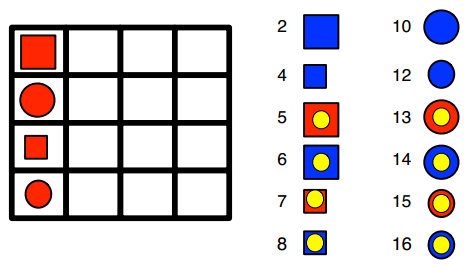
\includegraphics{pictures/win.png}
\caption[A \quarto{} win]{A winning board state in \quarto{}}
\end{figure}
The most obvious board-state to look for is a win, i.e. four pieces in a line  
sharing at least one attribute. To do this we compare all the pieces in each 
row, column and diagonal with each other and if a line is found where all 
pieces are equal we return a value of 100.

\subsection{Ties}
\begin{figure}[htb]
\label{fig: tie}
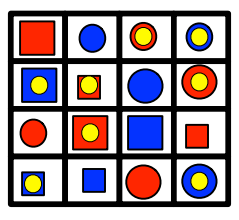
\includegraphics{pictures/tie.png}
\caption[A tie in \quarto{}]{A tied board state in \quarto{}}
\end{figure}
Another nice board-state to look out for is a tie, when all sixteen pieces have 
been placed on the board, but no win has been achieved. Checking this is merely 
counting if there are 16 pieces placed on the board, and if there is a  win. 
Since two optimal players will always tie\footnote{Proof of optimal play 
resulting in a tie: \url{http://web.archive.org/web/20041012023358/http://ssel.vub.ac.be/Members/LucGoossens/quarto/quartotext.htm}}, 
this is evaluated as 0, making sure that the minimax player will always 
choose a tie over a possible loss.

\subsection{Guaranteed losses}
\begin{figure}[htb]
\label{fig: gloss}
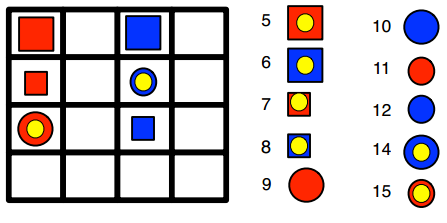
\includegraphics{pictures/gloss.png}
\caption[A guaranteed loss in \quarto{}]{A board state showing a guaranteed loss in \quarto{}}
\end{figure}
When there are two distinct 3-piece lines which have opposite values of at least 
one attribute, giving any piece to the opponent is a  guaranteed loss.
When we search for these states, we start of by finding all 3-piece lines on the 
board, then compare them to see if any of them have opposite values of an attribute.
Since a loss is the worst possible outcome of a game of \quarto{}, these states 
are valued at -100 in order to make the minimax player steer away from them.

\subsection{3-piece lines}
\begin{figure}[htb]
\label{fig: 3-odd}
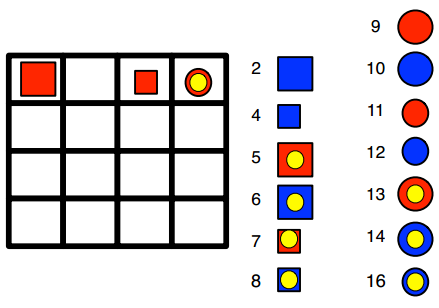
\includegraphics{pictures/3-odd.png}
\caption[A 3-piece line in \quarto{}]{A board state showing a 3-piece line with 
an odd number of winning pieces}
\end{figure}
\begin{figure}[htb]
\label{fig: 3-even}
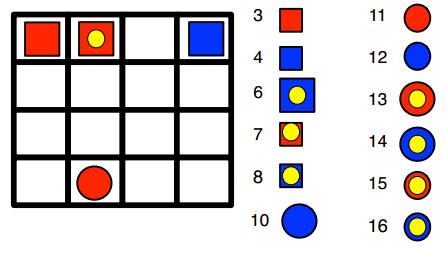
\includegraphics{pictures/3-even.png}
\caption[A 3-piece line in \quarto{}]{A board state showing a 3-piece line with 
an even number of winning pieces}
\end{figure}
A board containing multiple 3-piece lines makes it difficult to give the 
opponent a non-winning piece to play. However, depending on whether there is 
an odd or even number of pieces that can be placed in the final slot of a 
3-piece line, is it possible to force the opponent into returning a winning 
piece. Since this is a risky strategy, the 3-piece lines with an even number 
of winning pieces are weighted heavier than the 3-piece lines with an odd 
number of winning pieces.

%TODO: include pictures


\section{Tournament}\label{tournament}
%TODO: needs to be written.

\section{Results}\label{results}

\subsection{Local}\label{results:local}

\subsection{Tournament}\label{results:tournament}


\section{Future work}\label{future work}
Our implementation is far from perfect and there are some improvements
that we came up with that we did not have time to implement. Below
are a few of the thoughts that we had for further improvements.

\subsection{Guaranteed losses}
There are cases of guaranteed losses that we do not currently detect, for 
instance: a 3-piece line of squares and one with red pieces, with only 
square and red pieces remaining to be placed(see figure \ref{fig:gloss2}).

\begin{figure}
	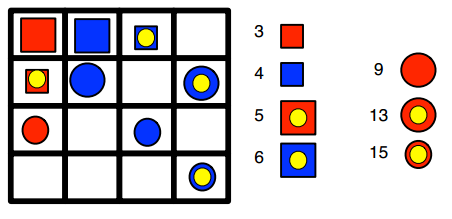
\includegraphics{pictures/gloss2.png}
	\caption{Another guaranteed loss situation not detected by
	our algorithm}
	\label{fig:gloss2}
\end{figure}


\appendix
\lstset{language=bash, frame=single, breaklines=true}
\lstloadlanguages{bash}
\section{Run configuration}\label{run configuration}
We have included our parameters below for the different results that we got
in the result section(see section \ref{results}). This should enable anyone to clone
our git repository and get about the same results out.

\begin{lstlisting}[label=lst:novice vs random, caption=Novice compared to random
player with 500 games]
$ python main.py game --player1 random --player2 novice -r 500 -s
\end{lstlisting}

\begin{lstlisting}[label=lst:novice vs minimax, caption=Novice compared to
minimax player with 500 games]
$ python main.py game --player1 minimax 3 6 --player2 novice -r 500 -s
\end{lstlisting}

\begin{lstlisting}[label=lst:minimax3 vs minimax4, caption=Minimax with a
depth of 4 compared to a minimax player with a depth of 3]
$ python main.py game --player1 minimax 3 6 --player2 minimax 4 6 -r 500 -s
\end{lstlisting}

\lstinputlisting[label=lst:switch code, caption=
Code to test most minimax depth against each other]{graphs/test_minimax_depth.sh}


\end{document}
